\documentclass[12pt]{article}
\usepackage[utf8]{inputenc}
\usepackage[margin=1in]{geometry} % Margins
\usepackage{authblk}  % Authors and Affiliations
\usepackage{fancyhdr} % Headers
\usepackage[parfill]{parskip}
\usepackage[inline]{asymptote}
\usepackage{amsmath}
\usepackage{hyperref}
\usepackage{float}
\usepackage{pdfpages}
% \usepackage[t,lf]{spectral}
\usepackage[T1]{fontenc}

\pagestyle{fancy}
\fancyhf{}
\fancyhead[L]{Zhang et al.}
\rhead{\thepage}

\begin{document}
% \includepdf[pages=1]{titlepage.pdf}

\begin{titlepage}
\raggedright


\includegraphics[width=0.2\textwidth]{images/tjlogo.png}

\Huge 
\textbf{Sentiment Distribution Analysis of News Headlines using Natural Language Processing and ANOVA Techniques}

\vspace{0.5cm}
\small
Final Project - \today

\vspace{1.5cm}
\large
\textbf{Athan Zhang} \hfill 1570738 \\
\textbf{Aidan Li} \hfill 1562961 \\
\textbf{Amy Wang} \hfill 1560918 \\

\vspace{1cm}
\small
Torbert Research Statistics,\\
Thomas Jefferson High School for Science and Technology

\vfill
\large
\textbf{Abstract} \\
\vspace{0.25cm}
\small
Sentiment analysis plays a crucial role in understanding public opinion and sentiment towards various topics. This study presents an application of Natural Language Processing (NLP) techniques combined with Analysis of Variance (ANOVA) to analyze sentiment in news headlines. The objective is to gain insights into the overall sentiment and identify any significant differences in sentiment across different news categories and publishers.

\vspace*{1cm}


\end{titlepage}

\tableofcontents
\newpage

\section{INTRODUCTION}

\subsection{Rationale}

Mean World Syndrome is a perceived cognitive bias in which people tend to see the world as cruel, a feeling that is amplified by repeated negativity in media. However, whether or not the media tends to trend more negatively in their reporting is unknown. This project aims to consider different variables that may affect the sentiment of news headlines in order to understand what really affects how positive or negative a news report can be. 

We use Natural Language Processing (NLP) techniques in order to extract sentiment data from headlines. These headlines are gathered from large public datasets that contain information on news articles, their headlines, category, date, and other variables covered later in this report. We are able to extract information on polarity (negative or positive) and subjectivity (opinionated or factual) to understand the sentiments of news headlines. 

To understand the statistical significance of the sentiment, we use Analysis of Variance techniques to see whether or not news headline sentiment and other variables, such as publisher and category, are homogenous in their distributions. This allows us to understand what variables play the largest role in news sentiment. 


\subsection{Related Works}

People interact with news reports on various social media platforms every day. In an investigation conducted in 2022, researchers detected positive and negative sentiments, as well as basic emotions like anger, disgust, fear, joy, sadness, and surprise. They found increasingly negative sentiment over time, with right-wing outlets being more harmful than left-wing outlets on average. In terms of specific emotions, they observed an increased proportion of headlines with anger, fear, disgust, and sadness \cite{rozado2022}.

Similarly, another article discusses the role of affect and emotion in successful viral diffusion, suggesting that effectively charged viral messages are more likely to spread than neutral ones. However, the article also contrasted these findings and established research on news factors, emphasizing adverse effects promoting propagation in news media. The methodology involves using machine learning techniques and applying them to different text corpora to classify messages as "news" and analyze sentiment \cite{hansen2011}.

BERT is an excellent example of machine learning that is used for this purpose. It can be used to analyze the sentiment involved within phrases and words, leading to the examination of how people react to differently worded posts about the same incident on multiple social media platforms. The model identifies emotions involved in a sequence of words to output. BERT was able to successfully pass the GLUE benchmark, shedding credibility to the language interpretation model \cite{devlin2019}.

In an article written in 2020, researchers tried using entity sentiment analysis that differentiates sentiment towards target entities and considers associated entities instead of using traditional methods. Their findings reveal the manner of sentiment expression and the specific aspect of the entity impacts sentiment strength. The study provides insights for improving entity sentiment analysis in news contexts by considering associated entities and sentiment expression and addressing the presence of biased entities \cite{luo2020}.

Researchers attempted to classify news articles and categorize them with viewer engagement. They were able to successfully predict how viewers would react to different types of posts on various social media platforms through past comments and analyzing the sentiments toward corresponding posts \cite{aldous2022}.


\subsection{Research Question}

Will the publisher or category of news headlines affect the polarity and subjectivity of them?

The goal of this research project is to find which variables such as publisher or category, have a relationship with the polarity and subjectivity of news headlines. 

\section{DATASET AND FEATURES}

We use two of the most widely used datasets for news headlines: the \textit{UCI News Aggregator} (NAD) and \textit{All The News} (ATN) datasets. Table \ref{tab:datasets} provides an overview of the datasets. More information can be found later in this section.

\begin{table}[H]
    \centering
    \begin{tabular}{|c|c|p{7cm}|}
        \hline
        \textbf{Dataset} & \textbf{Instances} & \textbf{Variables}   \\
        \hline
        News Aggregator & 422,419 & 4 \newline (Headline, Publisher, Category, Date) \\ 
        All The News & 142,568 & 3 \newline (Headline, Publisher, Date)\\
        \hline
    \end{tabular}
    \caption{Dataset Information}
    \label{tab:datasets}
\end{table}

NAD will be used to analyze the effect of \textit{Category} on Polarity, and thus the bar chart for categories can be seen in Figure \ref{fig:NAD_Category_Bar}. It will also be used to explore the relationship between Polarity and Subjectivity.

\begin{figure}[H]
    \centering
    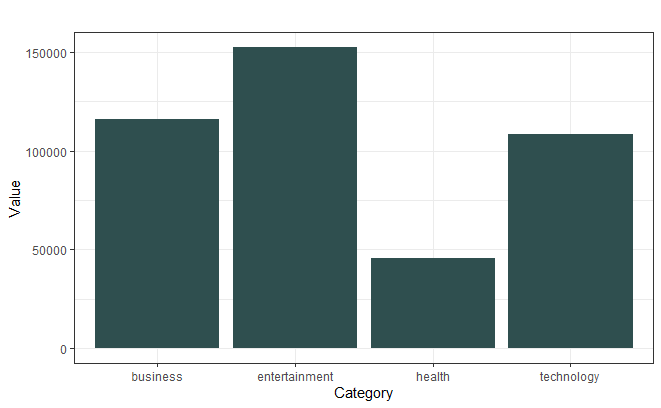
\includegraphics[width=0.7\textwidth]{images/NAD_Category_Bar.png}
    \caption{Bar Chart of Categories for NAD}
    \label{fig:NAD_Category_Bar}
\end{figure}

ATN will be used to analyze the effects of \textit{Publisher} on Polarity, and thus the respective bar chart is shown in Figures \ref{fig:ATN_Publisher_Bar}.

\begin{figure}[H]
    \centering
    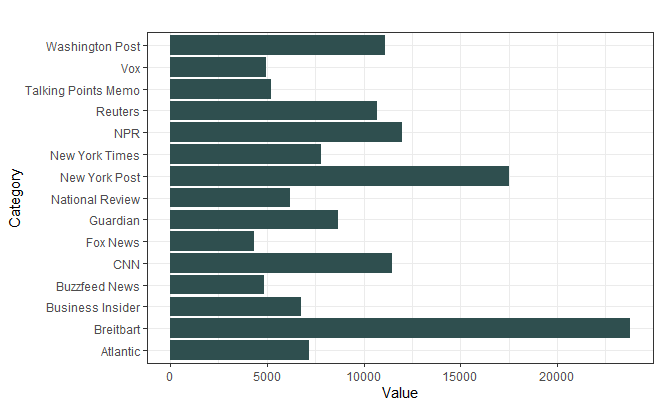
\includegraphics[width=0.7\textwidth]{images/ATN_Publisher_Bar.png}
    \caption{Bar Chart of Publishers for ATN}
    \label{fig:ATN_Publisher_Bar}
\end{figure}

Each dataset was chosen for its respective strengths. The NAD dataset allows us to get a comprehensive overview of categories, while the ATN dataset provides a large yet concise analysis of different major media corporations. 

More data analysis on Polarity and Subjectivity will be provided later in the Results section of this report.

\subsection{News Aggregator Dataset}

The News Aggregator Dataset (NAD) is provided by the University of California Irvine's Machine Learning Repository \cite{dua2019}. It is curated initially from understanding user interests based on web activity \cite{gasparetti2016}. 

The dataset is extensive and supplies a large amount of news article data. A primary variable of interest is the 'Category' variable, which allows us to explore disparities between different reporting focuses and their effect on sentiment. The main primary drawback of this dataset is its short timeframe, only pulling news data from 2014. 

\subsection{All The News}

The All The News dataset is made publicly available by Kaggle. It is a web-scraped collection of news headlines from late 2015 to 2017. The data wasn't subject to random sampling and data collection was made at the curator's discretion \cite{thompson2017}.

This dataset allows for a smaller range of different publishers but highlights major news corporations of interest such as The New York Times, CNN, Vox, Buzzfeed, etc. It also has a larger time frame which allows us to view changes in sentiment over time. However, this dataset did not group headlines by category, so there will be more data exploration within that variable. 

\section{METHODS}

\subsection{Analysis of Variance (ANOVA)}

ANOVA, which stands for \textit{Analysis of Variance}, is a statistical method used to analyze the differences between the means of three or more groups. It helps determine if there are significant variations among the group means and whether those differences are due to random chance or actual group differences. The formula for one-way ANOVA is:

\[
F = \frac{{\text{{between-group variance}} / (\text{{number of groups}} - 1)}}{{\text{{within-group variance}} / (\text{{total number of observations}} - \text{{number of groups}})}}
\]

The between-group variance measures the variation between the means of different groups, while the within-group variance measures the variation within each group. By comparing these variances, the F-ratio is calculated. If the F-ratio exceeds a certain critical value, it indicates that the group means are significantly different from each other, suggesting that there is a significant effect of the independent variable on the dependent variable.


\subsection{Natural Language Processing}

Natural Language Processing (NLP) is a field of study that combines linguistics, computer science, and artificial intelligence to enable computers to understand, interpret, and generate human language. It focuses on developing algorithms and models to process and analyze textual data. NLP encompasses various tasks, such as sentiment analysis, text classification, named entity recognition, machine translation, and question answering. Techniques like tokenization, part-of-speech tagging, syntactic parsing, and word embeddings are commonly used in NLP.

We used NLP techniques to analyze the headlines and generate polarity and subjectivity scores.
\begin{itemize}
    \item Polarity: A range between -1 and 1 is used to measure positive or negative sentiment, positive being higher values.
    \item Subjectivity: A range between 0 and 1 and refers to personal opinions and judgments.
\end{itemize}

TextBlob is an open-sourced Python library that makes sentiment analysis simple. We tokenized each headline in the datasets and generated their respective polarity and subjectivity scores using TextBlob \cite{loria2018}. This was then used as our response variable of the study and a primary focus variable.

\subsection{Implementation}

The proposed approach was implemented on Python 3.6. and R 4.3.

\begin{itemize}
    \item \textbf{GitHub Repository:} 
    \newline
    \url{https://github.com/athanzxyt/newsheadline_sentiment}
\end{itemize}

We used NumPy and Pandas Python data-processing libraries. TextBlob for Sentiment Analysis. Matplotlib and ggplot2 for Data Visualization. and Mosaic and RTools for statistical analysis.

\section{RESULTS \& DISCUSSION}

\subsection{Polarity \& Subjectivity Calculations}

The calculated Polarity and Subjectivity scores are calculated for the two datasets. The descriptive statistics are shown in Table \ref{lab:desc_stats} and the distributions in Figure \ref{fig:PS_histos}. 

\begin{table}[H]
    \centering
    \begin{tabular}{lcccc}
    \hline
                             & \multicolumn{2}{c}{NAD} & \multicolumn{2}{c}{ATN} \\
                             & Polarity & Subjectivity & Polarity & Subjectivity \\ \hline
    \multicolumn{1}{l|}{$\mu$}  & 0.043    & 0.224 & 0.030    & 0.256 \\
    \multicolumn{1}{l|}{$\sigma$}  & 0.222    & 0.297 & 0.241    & 0.307 \\
    \multicolumn{1}{l|}{Max} & 1.000    & 1.000 & 1.000    & 1.000 \\
    \multicolumn{1}{l|}{Q3}  & 0.080    & 0.455 & 0.100    & 0.455 \\
    \multicolumn{1}{l|}{Med} & 0.000   & 0.000 & 0.000    & 0.100 \\
    \multicolumn{1}{l|}{Q1}  & 0.000   & 0.000 & 0.000    & 0.000 \\
    \multicolumn{1}{l|}{Min} & -1.000       & 0.000 & -1.000       & 0.000 \\
    \hline
    \end{tabular}
    \caption{Descriptive Statistics for Polarity and Subjectivity Scores}
    \label{lab:desc_stats}
\end{table}

We can see that the max, minimum, and first quartile are the same between NAD and ATN. Mean-wise, NAD has a greater mean for polarity compared to ATN, while ATN has a greater mean for Subjectivity than NAD. The opposite is true for the standard deviations. The quartile 3 for polarity at ATN is slightly higher than the one at NAD. For the median, the subjectivity for ATN is slightly more significant than NAD.

\begin{figure}[H]
    \centering
    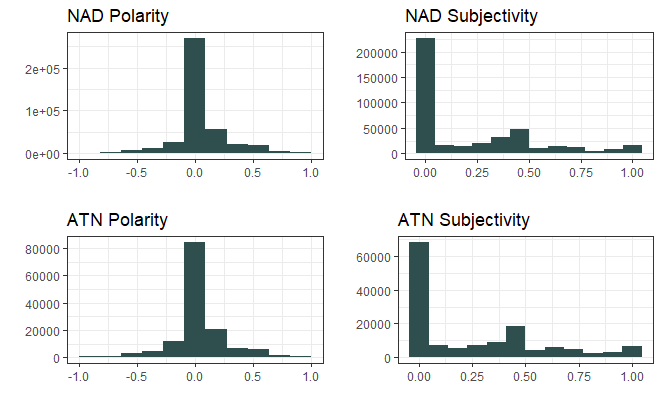
\includegraphics[width=0.9\textwidth]{images/PS_histos.png}
    \caption{Histograms for Polarity and Subjectivity}
    \label{fig:PS_histos}
\end{figure}

We can determine that the histograms for polarity and subjectivity, each, are relatively similar. Between the NAD and ATN polarity, the histograms are centered around 0 and have a relatively normal distribution. However, for the NAD and ATN subjectivity histograms, the mean seems to be near 0 with both graphs being extremely right-skewed.

Further explanatory data analysis is conducted. We plot the scatterplots of Polarity versus Subjectivity and the absolute value of Polarity versus Subjectivity in Figures \ref{fig:PolSub_NAD} and \ref{fig:PolSub_ATN}.

\begin{figure}[H]
    \centering
    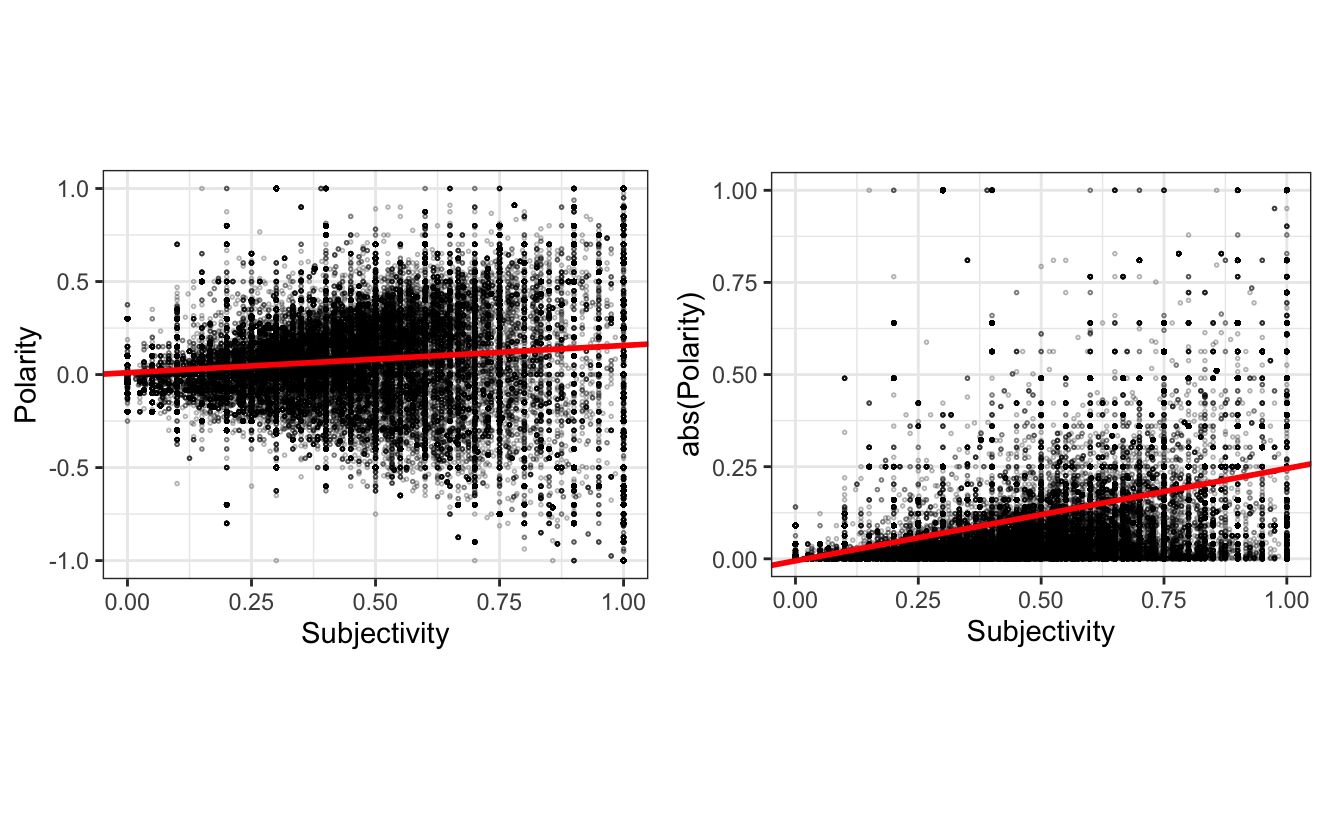
\includegraphics[width=0.8\textwidth]{images/PolSub_NAD.png}
    \caption{Polarity versus Subjectivity Scatterplot for NAD}
    \label{fig:PolSub_NAD}
\end{figure}

\begin{figure}[H]
    \centering
    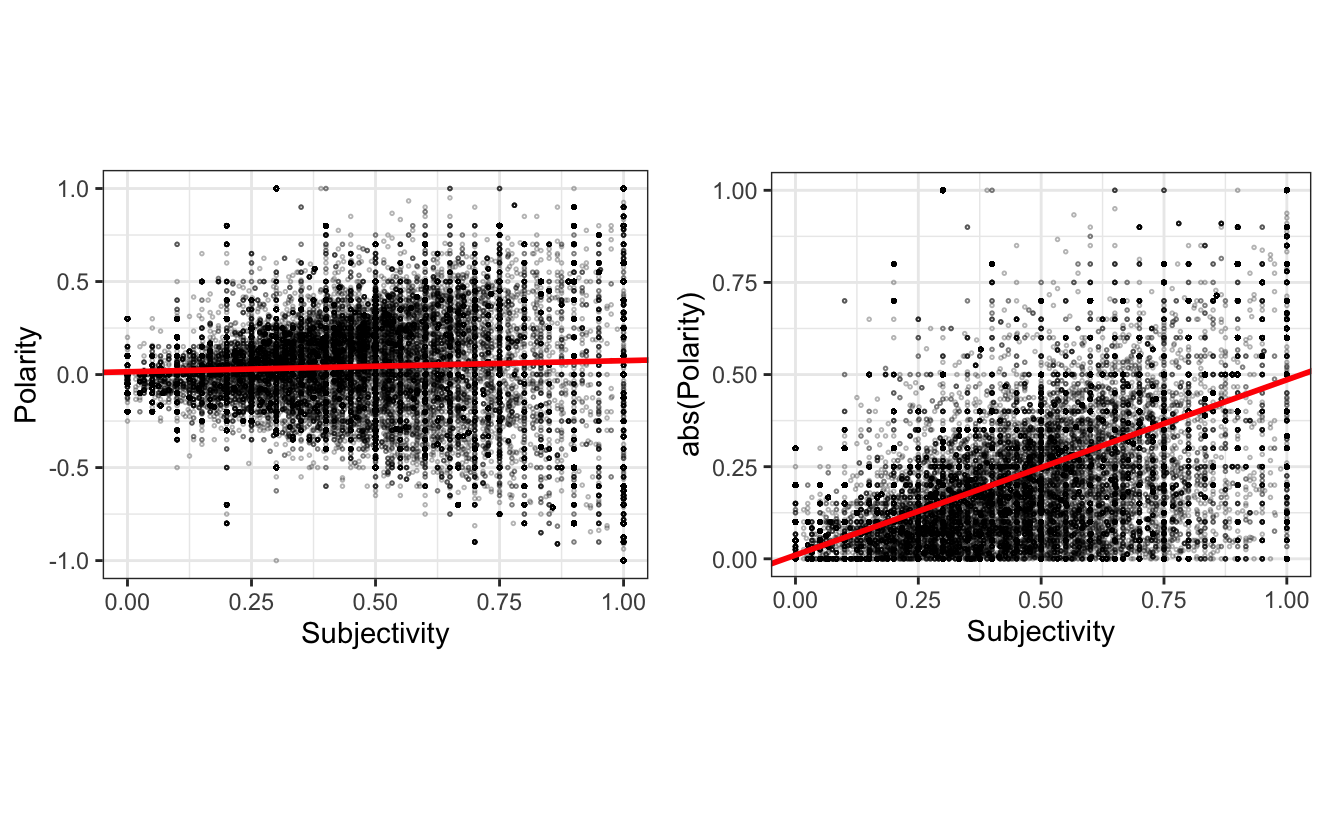
\includegraphics[width=0.8\textwidth]{images/PolSub_ATN.png}
    \caption{Polarity versus Subjectivity Scatterplot for ATN}
    \label{fig:PolSub_ATN}
\end{figure}

As we can see, the relationship between Polarity and Subjectivity seems to be relatively apparent, with a moderate linear positive relationship. However, since the variance of Polarity increases with Subjectivity, we did not carry out regression tasks. Nevertheless, an interesting observation that as news headlines become more subjective, they tend to become more extreme in their sentiments.

\subsection{Category and Polarity}

We first explore the relationship between the category of the news headline on its polarity. We examined four categories: technology, health, entertainment, and business-related news headlines. The distributions of this can be seen in Figure \ref{fig:CatPol_Dist}.

\begin{figure}[H]
    \centering
    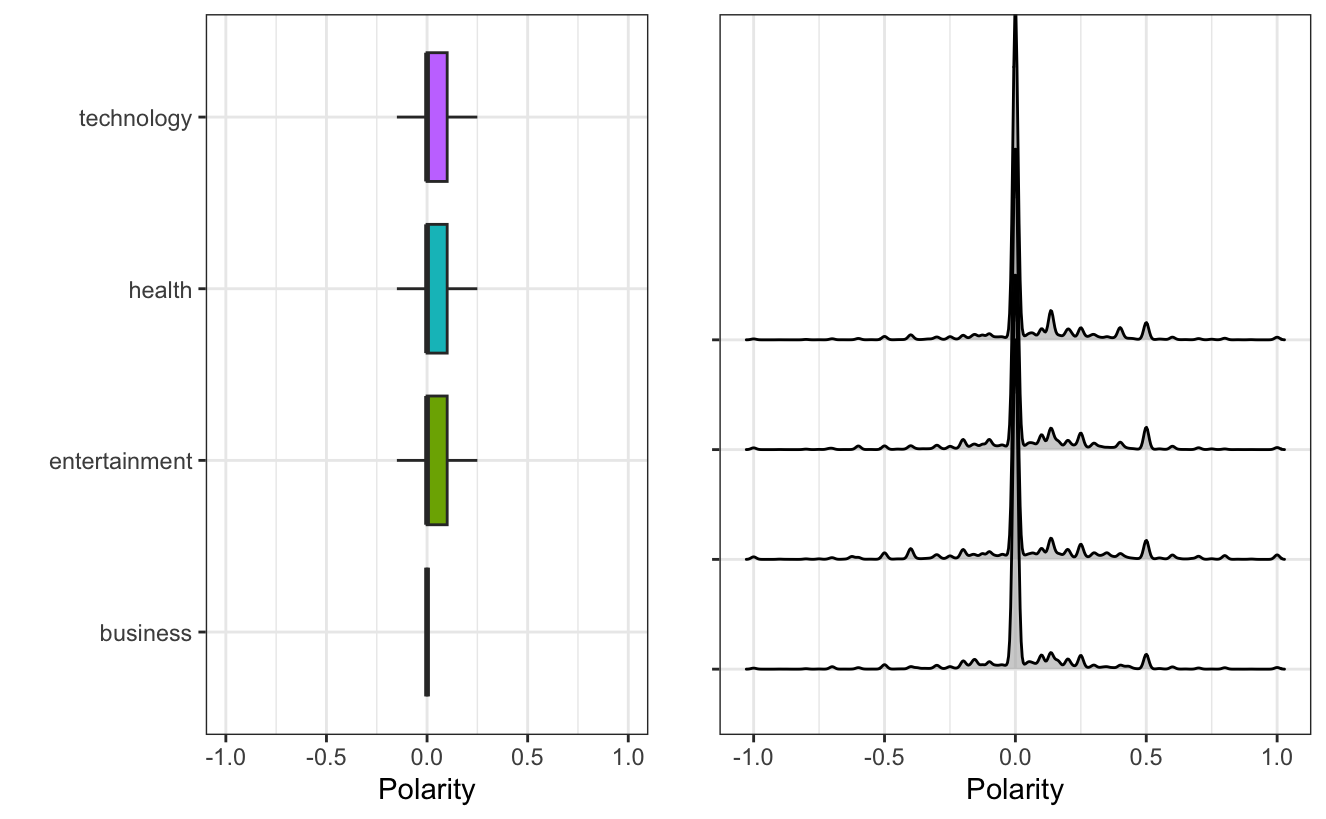
\includegraphics[width=1\textwidth]{images/CatPol_Dist.png}
    \caption{Polarity Distributions of each Category in NAD}
    \label{fig:CatPol_Dist}
\end{figure}

All distributions appear to be symmetric and approximately normal. All distributions appear to have similar shapes, with the exception of the business category, which has its entire boxplot located at zero. All outliers were removed for the sake of visualization.

Since our dataset meets the independent condition (there are likely more than one million news articles from 2014), is generated from observation, and appears to be approximately normal (distributions and also generated from a significantly large dataset), we continue with a one-way ANOVA test of homogeneity. The hypothesis of the test can be found below.

\begin{center}
    $H_{0}$: $\mu_{t}$ = $\mu_{h}$ = $\mu_{e}$ = $\mu_{b}$ \\
    $H_{a}$: \text{At least one of}\;$\mu_{k}$\;\text{differs}\\
\end{center}

Where $\mu_{k}$ represents the true mean polarity for each category. The results of the ANOVA can be found below.

\begin{table}[H]
    \centering
    \begin{tabular}{|llllll|}
    \hline
                                    & DF     & Sum Sq  & Mean Sq & F-Value & P       \\ \cline{2-6} 
    \multicolumn{1}{|l|}{Category}  & 3      & 29.8    & 9.9473  & 202.52  & 2.2E-16 \\
    \multicolumn{1}{|l|}{Residuals} & 422415 & 20747.5 & 0.0491  &         &         \\ \hline
    \end{tabular}
\end{table}

As we can see, we have a relatively high F-value which suggests that the means are not necessarily all equal. This is furthered by the p-value of 2.2E-16, which is less than $\alpha = 0.05$; thus, we reject the null hypothesis. There is statistical evidence that one of the news headline categories does not have the same mean polarity.

Conducting a Fisher LSD procedure finds that technology and business are individual groups, while entertainment and health share a similar mean polarity.

\subsection{Publisher and Polarity}

The polarities are displayed graphically with side-by-side density and dot plots in Figure \ref{fig:PubPol_Dist}. We can see that all distributions appear to be relatively symmetric with similar spreads, with the exception of the New York Times. 

\begin{figure}[H]
    \centering
    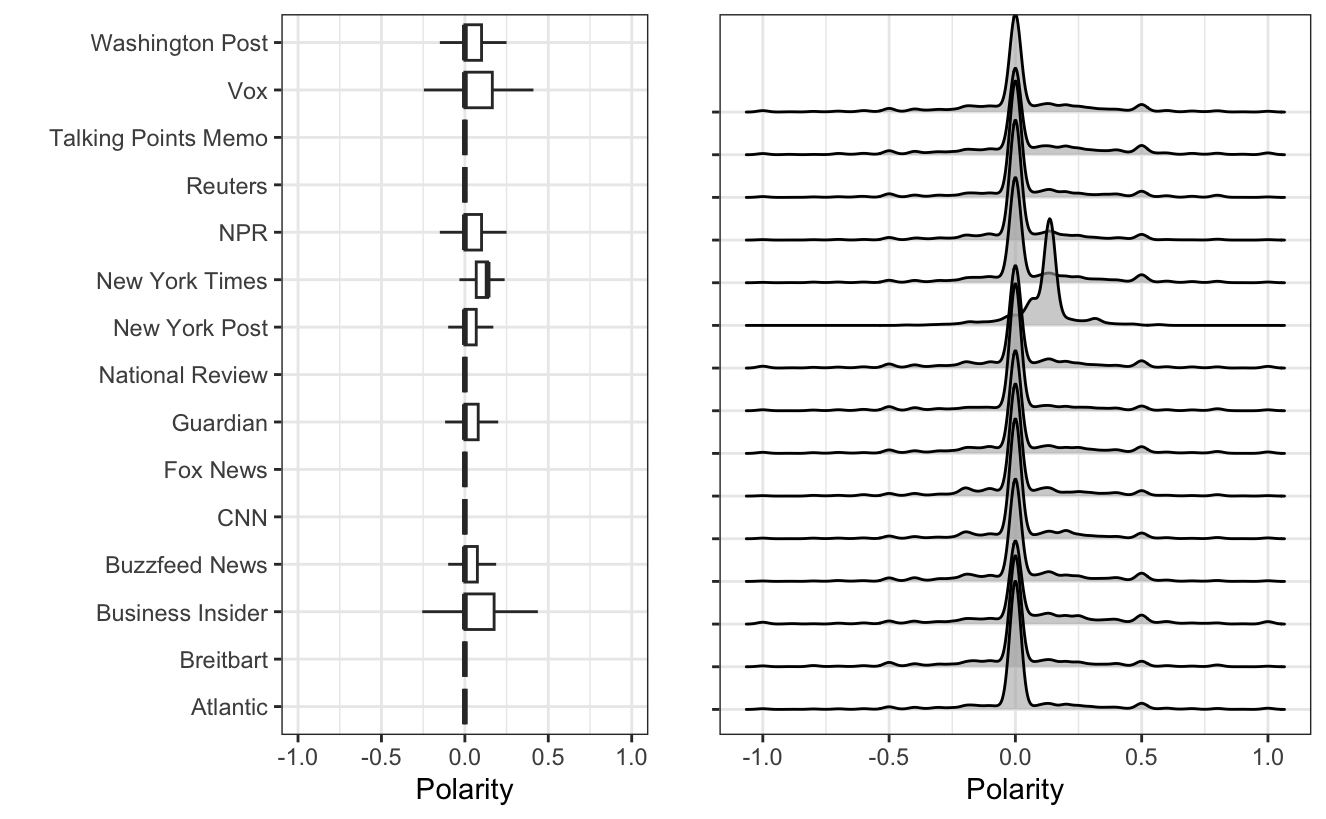
\includegraphics[width=1\textwidth]{images/PubPol_Dist.png}
    \caption{Polarity Distributions of each Publisher in ATN}
    \label{fig:PubPol_Dist}
\end{figure}

Analyzing the density graphs, we can see that all of the graphs are centered around a polarity of 0 with a normal distribution, save for New York Times. New York Times has a slightly greater polarity mean as it is shifted to the right of all the other density graphs. As the box plots show, noting that all outliers have already been removed, the publishers all have varying variances. For example, Talking Points Memo, Reuters, National Review, Fox News, CNN, Breitbart, and Atlantic all are centered on a polarity of 0, with almost no variance at all. New York Times, New York Post, Guardian, and Buzzfeed News have a similar range, mostly around 0.25. However, the other publishers all have a relatively high variance, with Business Insider having a range nearing 0.75.

Since our dataset meets the independent condition (there are likely more than one million news articles from 2015-2017), is generated from observation, and appears to be approximately normal (distributions and also generated from a significantly large dataset), we continue with a one-way ANOVA test of homogeneity. The hypothesis of the test can be found below.

\begin{center}
    $H_{0}$: $\mu_{WaPo}$ = $\mu_{Vox}$ = ... = $\mu_{Atlantic}$ = $\mu_{CNN}$ \\
    $H_{a}$: \text{At least one of}\;$\mu_{k}$\;\text{differs}\\
\end{center}

Where $\mu_{k}$ represents the true mean polarity for each publisher. The results of the ANOVA can be found below.

\begin{table}[H]
    \centering
    \begin{tabular}{|llllll|}
    \hline
                                    & DF     & Sum Sq & Mean Sq & F-Value & P       \\ \cline{2-6} 
    \multicolumn{1}{|l|}{Category}  & 14     & 78.4   & 5.5992  & 97.592  & 2.2E-16 \\
    \multicolumn{1}{|l|}{Residuals} & 142551 & 8178.6 & 0.0574  &         &         \\ \hline
    \end{tabular}
\end{table}

As we can see, we have a relatively high F-value which suggests that the means are not necessarily all equal. This is furthered by the p-value of 2.2E-16, which is less than $\alpha = 0.05$; thus, we reject the null hypothesis. There is statistical evidence that one of the news headline categories does not have the same mean polarity.

Conducting a Fisher LSD procedure aids us in identifying which publishers have similar means. Figure \ref{fig:relationships} shows a relationship map of these groups.

\begin{figure}[H]
    \centering
    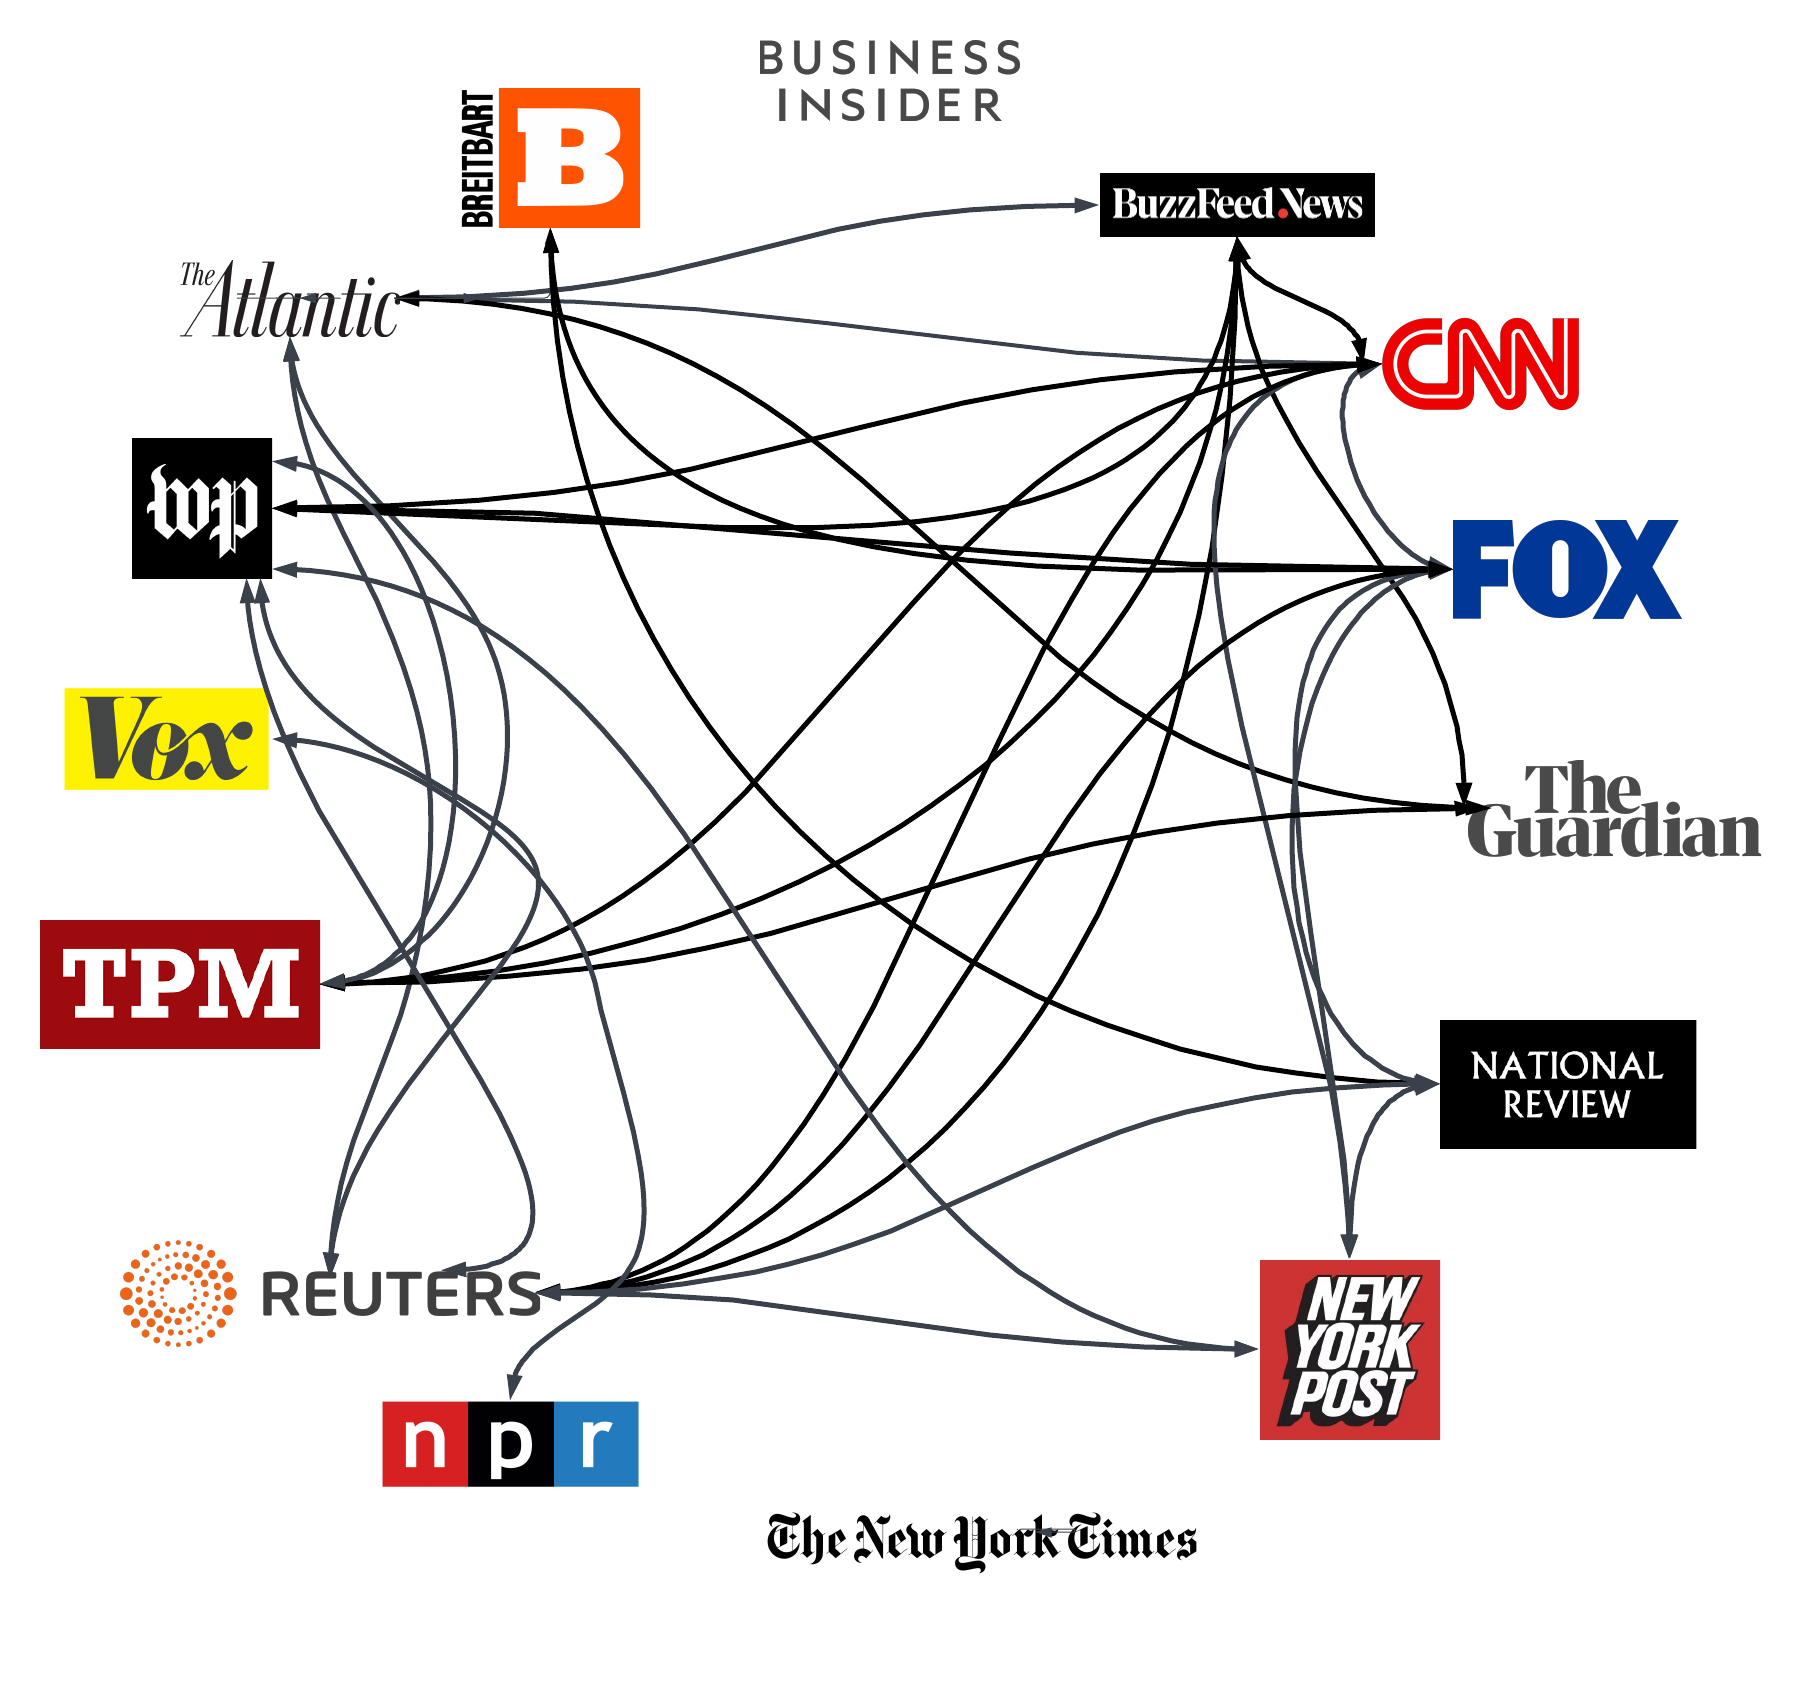
\includegraphics[width=1\textwidth]{images/relationships.png}
    \caption{Shared Polarity Means among Publishers}
    \label{fig:relationships}
\end{figure}

Most notably, two news sources were not a part of any group: The New York Times and Business Insider. As seen from the previous boxplots, this is most likely indicative of a more positive polarity than the other news sources. Other groups, however, saw multiple news sources having similar average polarities. While traditionally right-leaning news sources were often grouped with traditionally right-leaning news sources and traditionally left-leaning news sources were frequently grouped with traditionally left-leaning news sources, there was a significant grouping of both left and right-leaning sources together. For example, while traditionally right-wing New York Post was correlated with other right-leaning sources like Breitbart, National Review, and Fox, it was also considered in the same group the Washington Post and CNN, both left-leaning news sources.

\section{CONCLUSION}

This report analyzes the polarity of news headlines on a variety of factors. We explored how the category of the news article, as well as the publisher of the news article, affects the sentiment of the headline.

We found a statistical difference in the polarity of news headlines across different news categories. This means that not all news categories are equally positive or negative. Most notably, we found that the business and technology categories are independent of health and entertainment, which share similar polarity scores. 

We also found a statistical difference in the polarity of news headlines across different news publishers. This means that different news corporations tend to publisher different sentiment headlines than others. Most notably, both Business Insider and The New York Times shared no statistically standard polarity score with other groups. From the density distributions, we note that the New York Times tends to publisher more positive news headlines. We provide information on which of the top news publishers publish similar sentiments in their headlines. 

We also noted an observational positive linear relationship between the polarity and subjectivity of news headlines. Most notably, as the subjectivity of a news headline increases, so does the extreme of its polarity. This reinforces the obvious idea that subjectivity results in bias, which results in extreme sentiments. 

\subsection{Connections to literature}

Similar to the results found in Rozado et al. (2022), Hansen et al. (2011), Aldous et al. (2023), we found that, with machine learning, we were able to find correlations between polarity involved in the news headlines and the company that published the bar, as well as the correlation between polarity and the category the news headline was in. When comparing polarity and subjectivity, we noticed a positive linear trend between the two.

\subsection{Further Research}

Some future work for this project is to increase the data pulled and analyzed. Being able to extensively analyze news headlines over multiple decades with millions of headlines will increase our analysis.

Additionally, improving the sentiment classification algorithm could result in more variables and information to analyze. Building multi-layered neural networks or using pre-trained BERT models could allow for deeper analysis.

This work could lastly be improved by expanding to the entire news article instead of simply just the headline; however, this is very computationally expensive and beyond the scope of this project. 

\subsection{Limitations}

There are a few notable limitations of this study that the authors want to note. First and foremost, the timeframes of the news articles collected span relatively short windows, reaching a timeframe of at max three years in some cases. The authors want to note potential biases and confounding variables that may be found in this window. However, nothing of notable significance occurred in these years, and sufficiently large amounts of data were pulled, mitigating some of these effects. 

Secondly, the categories analysis did not include a political category, which is a typically charged sentiment domain.

Thirdly, the groups across both datasets were not necessarily balanced; for example, there were notably fewer health news headlines than others from categories.

Finally, the sentiment measurement of polarity and subjectivity could be naturally biased based off of the dataset that the TextBlob classifier was trained on, which may be reflected in our calculations.

\subsection{Reflections}

During our project on analyzing news headlines using sentiment analysis, we developed several skills that could significantly enhance our capabilities as researchers and budding statisticians, which could prove valuable in future research endeavors. The first skill, of course, is statistical analysis: This project necessitated the use of various statistical techniques to analyze the sentiment of news headlines accurately. We gained proficiency in applying statistical methods such as hypothesis testing and the four-step process, as well as identifying areas of inquiry. These statistical analysis skills are fundamental for any researcher and can be applied to diverse research subjects. Furthermore, the project demanded extensive coding in R for data manipulation, visualization, and statistical modeling. Applying R to real-world applications has equipped us with a powerful tool for future research projects in each of our respective fields. For instance, when studying the impact of environmental factors on public health, we can utilize R to analyze large datasets, visualize trends, and build predictive models. The ability to program effectively will allow me to handle complex research tasks efficiently and automate processes that may have taken ages manually. While we had many successes, our failures were numerous as well. Throughout the project, we encountered several challenges, such as dealing with errors in RStudio, managing outliers, and selecting appropriate statistical methods. Overcoming these obstacles required critical thinking and problem-solving skills, as well as sheer determination to not give up at times. Finally, we learned significant lessons during the interpretation and communication of research findings. We learned how to analyze and summarize the sentiment trends in news headlines and present the results in a clear and concise manner.

\section{ACKNOWLEDGEMENTS}

This research did not receive any specific grant from funding agencies in the public, commercial, or not-for-profit sectors. 

The authors would like to thank Dr. Shane Torbert of the Thomas Jefferson High School for Science and Technology (TJHSST) for his invaluable contributions in field knowledge and manuscript review.

\bibliographystyle{apalike}
\bibliography{refs}

\end{document}
